
%----------------------------------------------------------------------------------------
% APPENDICES
%----------------------------------------------------------------------------------------

\appendix
\pagelayout{wide}
\addpart{Appendices}

\pagelayout{margin}
\setchapterstyle{kao}
\chapter{The Setup Guide}\label{app:setup}
This appendix helps you install packages and configure the accounts used by the chapter examples. Begin with the setup for the example you intend to run; an example using a dataset supplied with Stata does not require Google or an LLM account. After setup, run that example from its first line and retain the log so you can distinguish an installation problem from a problem in the analysis.

\paragraph{Packages.} The companion \texttt{01\_install.do} installs the core community and book packages. Optional installations, including \texttt{googlesheets}, \texttt{googlechart}, and the dashboard tools, are commented out; remove the leading comment marker from the installation lines needed for your example. Each chapter's Package Integration box gives its installation commands, and Appendix~\ref{app:toolkit} provides a package guide. If Stata reports \enquote{command unrecognized}, use \texttt{which} followed by the command name to check whether Stata can find it. If the installation failed, read the earlier download error in the log before repeating it.

\paragraph{API keys and \texttt{profile.do} hygiene.} Several sources need a free key. Request them once (Census at \texttt{api.census.gov/data/key\_signup.html}; FRED at \texttt{fred.stlouisfed.org}), then store them where shared code will never see them:
\begin{itemize}
    \item Put \texttt{global censuskey "YOUR\_KEY"} in your \texttt{profile.do}, which Stata runs at startup, so the key loads automatically and stays out of your do-files.
    \item For FRED, run \texttt{set fredkey YOUR\_KEY, permanently} once; Stata remembers it.
    \item Never paste a key into a do-file you will commit to a repository. A key in public version control is a key someone else will spend, and deleting it in a later commit does not help: git keeps every past commit, so anyone with a copy of the repository can still read the key out of its history. If a key does reach a repository, revoke it at the provider and reissue a new one, because that is the only step that actually ends the exposure; tools like \texttt{git-secrets} or GitHub push protection catch the mistake before the push.
\end{itemize}

\paragraph{Python: two different arrangements.} Two kinds of tools in this book use Python, and they ask different things of you, so it is worth separating them once. The book's LLM examples run through Stata's own Python integration. Check which interpreter Stata sees with \texttt{python query}, and keep project dependencies in a virtual environment so one project's package versions do not disturb another's. One compatibility note applies only to this route: Stata talks to Python over a shared C API, so the interpreter must be a shared-library build (\texttt{--enable-shared}); the stripped Pythons some package managers ship will pass \texttt{python query} yet fail to load, and \texttt{python set exec} lets you point at a working one. The web-API tools take the other arrangement and ask less. \texttt{webapi} and \texttt{googlesheets} each run a helper script with the \texttt{python3} already on your system path rather than through Stata's integration, so the only requirement is that \texttt{python3} answers when you type \texttt{shell python3 -{}-version}. \texttt{webapi} needs nothing beyond Python's standard library; \texttt{googlesheets} needs Google's client libraries and installs them itself, into a private environment it builds on first run, so you never manage those packages by hand.

\paragraph{Google Cloud OAuth for \texttt{googlesheets}.} Because \texttt{googlesheets} reads and writes documents that belong to you, Google has to be satisfied that the commands really are acting on your behalf. The setup below arranges exactly that: you authorize this copy of Stata, once, to act as you inside your own account. It takes six steps, done once per machine.
\begin{enumerate}
    \item Create a free project at \texttt{console.cloud.google.com}; any name will do. The project is only a container Google uses to track the permission you are about to grant.
    \item Inside that project, switch on both the Google Sheets API and the Google Drive API. Stata calls both, so enabling one and not the other is the most common reason a first run fails.
    \item On the consent screen, choose \emph{External}, add your own Google address as a test user, and grant the two scopes the package needs, \texttt{.../auth/spreadsheets} and \texttt{.../auth/drive}. This is where you say which account Stata may act as, and what it may touch.
    \item Create credentials of type \emph{Desktop app} and download the small \texttt{.json} file Google gives you. That file identifies the package to Google; save it somewhere stable, such as \texttt{\~{}/.config/stata-googlesheets/client.json}.
    \item Point Stata at that file with one global, \texttt{global GS\_CLIENT "\ldots"}. We suggest you put that line in your \texttt{profile.do} so you set the path once and never paste it into a script you share.
    \item Run any \texttt{googlesheets} command. A browser opens, you pick your account and click \emph{Allow}, and Stata saves a reusable token beside the credentials file. Every later call runs silently.
\end{enumerate}
\emph{OAuth} lets you authorize a program to act inside your account without giving it your password. The saved \emph{refresh token} lets the program renew access while that authorization remains valid. For an External app in \enquote{Testing} status using the Sheets and Drive scopes above, Google issues refresh tokens that expire after seven days.\marginnote{Google documents the Testing limit and other reasons tokens expire at \url{https://developers.google.com/identity/protocols/oauth2}, checked September 2026. The exception for basic identity scopes does not cover Sheets and Drive access.} An unattended weekly report can therefore stop even though its first run succeeded. Test renewal before scheduling the report, and arrange an authentication method your organization permits for unattended use. A service account, where the package supports it, needs permission to the particular files it will read or write. For a response sheet intentionally made readable without signing in, Chapter~\ref{ch:surveys} also shows a credential-free import.

\paragraph{LLM setup, hosted and local.} For hosted LLMs, install the vendor's SDK (for example \texttt{pip install google-genai}) and store the API key in an environment variable, never in a do-file. For protected data that cannot leave the building, install Ollama locally, pull an LLM (\texttt{ollama pull llama3} or a Gemma model), and confirm the local server is running before Stata calls it. Budget for the download: a quantized 7B LLM is 4--5\,GB and a laptop with 16\,GB of RAM can run it, but the larger LLMs that rival hosted quality need a GPU. Ollama serves on \texttt{localhost:11434} by default, so a \texttt{curl} to that port is the fastest check that the server is running. The LLM-agnostic wrapper of Chapter~\ref{ch:ai} lets you switch between the two by changing one macro.

\paragraph{Setup instructions for your team.} Once an example works on your machine, record its setup in \texttt{SETUP.md} or a commented header in \texttt{01\_install.do}. Include the required Stata version, packages, paths, and account permissions, then ask a colleague to follow those instructions on another machine. Where they stop, add the missing instruction and the expected result. This gives the next analyst a way to check the environment before changing working analysis code.

\pagelayout{margin}
\setchapterstyle{kao}
\chapter{The Causal Quick-Reference Toolbox}\label{app:causal}
Chapter~\ref{ch:claims} develops difference-in-differences (Section~\ref{sec:did}). Here we introduce related designs, the circumstances in which you might consider them, and Stata commands to investigate further. Begin by writing down how people or sites received the program, which outcomes you observe before and after it, and which untreated units could provide a comparison. A staggered rollout across districts may support difference-in-differences; an eligibility threshold may support regression discontinuity. Neither feature establishes a credible design by itself. Use the entries below to identify the assumptions you would need to defend, then consult the specialist references before estimating a program effect.

\begin{description}
    \item[Staggered treatment timing.] When units adopt a policy at different times, consider \texttt{csdid} (Callaway and Sant'Anna) or \texttt{jwdid} (Wooldridge). These approaches address problems that arise when plain two-way fixed effects uses already-treated units as comparisons and treatment effects change over time. Examine an event-study plot alongside your account of how the program was assigned. \emph{Caveat:} similar observed pre-trends cannot establish the parallel trends assumption for untreated outcomes after adoption.\marginnote{Goodman-Bacon's basic decomposition has nonnegative weights on the $2\times2$ comparisons. The problem is that some comparisons use already-treated units whose outcomes may still be changing because of treatment. Negative weights can arise in the separate representation in terms of underlying treatment effects. Adding leads and lags to a conventional two-way fixed-effects regression does not generally resolve this problem.}
    \item[Sharp eligibility cutoff.] When a rule assigns treatment at a threshold, regression discontinuity compares units just above and below it. Estimate with \texttt{rdrobust}, inspect the running variable's density with \texttt{rddensity}, and plot outcomes with \texttt{rdplot}. Check whether another policy also changes at the cutoff and whether applicants could precisely manipulate their position relative to it. \emph{Caveat:} a density test alone cannot establish that assignment was credible, and the effect is local to the cutoff.\marginnote{The bandwidth determines how far from the cutoff observations enter the local estimate. Report the selected bandwidth and the number of observations on each side, and examine sensitivity to reasonable alternatives. The robust bias-corrected interval accounts for estimating and correcting smoothing bias; it is not simply an interval widened because the bandwidth was selected from the data.}
    \item[A single treated unit.] When one state or site is treated, synthetic control (\texttt{synth}) uses a weighted combination of untreated units to approximate its pre-treatment outcome path. Compare the post-treatment gap with placebo gaps obtained by assigning treatment to donors, taking their pre-treatment fit into account. \emph{Caveat:} you need donors that provide a credible untreated comparison and are unaffected by the intervention.\marginnote{Inspect the donor weights and repeat the analysis after removing influential donors. A large weight on one donor is a reason to examine that donor's comparability, rather than automatic evidence of a failed match. A close pre-treatment fit can still be misleading if a donor experiences a different post-treatment shock.}
    \item[Panels with time-varying shocks.] Synthetic difference-in-differences (\texttt{sdid}) adds unit and time weights to a DiD, adjusting for pre-trends and common shocks at once. \emph{Caveat:} interpretability of the weights is a communication task in itself (Chapter~\ref{ch:graphs}).
    \item[Many measured covariates.] Double/debiased machine learning (\texttt{ddml}, with learners supplied through tools such as \texttt{pystacked}) can estimate the outcome and treatment relationships flexibly. Cross-fitting means that each observation receives predictions from learners fitted on other observations. The estimator also uses an estimating equation designed to reduce sensitivity to small errors in those predictions. These features do not remove unmeasured confounding: you still need a credible identification assumption, adequate overlap between treated and untreated units, and sufficiently accurate nuisance estimates. The statement that either of two correctly specified models suffices applies to particular doubly robust estimators, not to every double machine learning specification. For your application, consult the assumptions of the \texttt{ddml} model you select.\marginnote{Ahrens, Hansen, Schaffer, and Wiemann (2024) explain the models and cross-fitting in \emph{The Stata Journal}: \url{https://doi.org/10.1177/1536867X241233641}.}
    \item[Effects that differ by subgroup.] When the question is \enquote{for whom} rather than \enquote{on average,} Stata~19's \texttt{cate} estimates group-average effects for prespecified groups and for data-driven groupings of the predicted effect; causal forests \parencite{wager2018forests} are the machinery underneath. \emph{Caveat:} data-driven subgroups inherit the winner's curse, so shrink or validate before anyone funds the loudest cell (Section~\ref{ch08-sc-shrinkfx}).
    \item[Treatment that spreads.] When treated and comparison units can share the treatment, through siblings, shared staff, or neighboring markets, every design above quietly mismeasures the effect. The first answer is design, not estimation: compare units the program cannot reach, or compare at the level where the leaking stops. \emph{Caveat:} estimation under interference is a specialist field; \textcite{huber2023causal} devotes a chapter to it.
\end{description}

\paragraph{Sensitivity, not just point estimates.} Because parallel trends and unconfoundedness cannot be proven, bound them. The \texttt{honestdid} package (Rambachan and Roth) reports how large a trend violation would have to be to overturn a DiD finding, and Oster's \texttt{psacalc} gauges robustness to omitted-variable bias.\marginnote{Oster's rule of thumb is a useful anchor: a result survives if the selection on unobservables would have to exceed the selection on observables (her $\delta > 1$) to drive the effect to zero. Report the $\delta$, not just a reassuring word.} And when attrition differs between treated and comparison groups, the panel problem Chapter~\ref{ch:panels} diagnoses, \texttt{leebounds} \parencite{lee2009bounds,tauchmann2014leebounds} brackets the effect without pretending the dropouts were random. Applied researchers increasingly report these bounds rather than a bare pass/fail pre-trend test.

\paragraph{Further reading.} For applied depth beyond this map: \textcite{cunningham2021mixtape}, \emph{Causal Inference: The Mixtape}, for intuition and Stata/R code; \textcite{huntingtonklein2022effect}, \emph{The Effect}, for design-first reasoning in plain language; and \textcite{cameron2022microeconometrics}, \emph{Microeconometrics Using Stata} (Vol.~II), for the econometric treatment of treatment effects; and \textcite{huber2023causal}, \emph{Causal Analysis}, for the estimator-by-estimator treatment of these designs and their machine-learning extensions, written for graduate courses in R. These are where the designs sketched here become methods you can defend.

\pagelayout{margin}
\setchapterstyle{kao}
\chapter{The Book's Toolkit}\label{app:toolkit}
Use this appendix to find any tool the book uses and jump straight to the chapter that puts it to work. It lists every package and proposed tool in one place, so when you remember a capability but not its name you can recover both. Three of these packages, \texttt{webapi}, \texttt{googlesheets}, and \texttt{googlechart}, are published on SSC, so a single line installs each of them:
\par
{\footnotesize
\begin{verbatim}
ssc install webapi
ssc install googlesheets
ssc install googlechart
\end{verbatim}
}
The rest install from the authors' GitHub. One \texttt{net install} line does it, and you swap in the repository name for each package:
\par
{\footnotesize
\begin{verbatim}
local gh "https://raw.githubusercontent.com/ericabooth"
net install statashiny, ///
    from("`gh'/StataShiny-public/main/") replace force
\end{verbatim}
}
\begin{itemize}
    \item \texttt{StataShiny-public}
    \item \texttt{dashboardbuilder-stata-public}
    \item \texttt{webdoc2-stata-public} (also needs \texttt{ssc install webdoc} and a follow-up \texttt{net get webdoc2} for its header template; its Chapter~\ref{ch:portals} box shows all three lines)
\end{itemize}
The one exception is \texttt{sparkta2}, whose source is not yet released. The companion \texttt{01\_install.do} contains every one of these lines ready to run.

\paragraph{Published packages.}
\begin{itemize}
    \item \texttt{webapi} -- fetch an authenticated JSON web API into Stata as a dataset, standard-library Python only (Chapter~\ref{ch:apis}).
    \item \textbf{The fourteen packages built for this book}, each in its own \texttt{-stata-public} repository with tests and help: \texttt{projectbuilder} (scaffold the Chapter~\ref{ch:workshop} project layout), \texttt{combineall} (append, merge, or convert a whole folder, with vintage-aware harmonization; Chapters~\ref{ch:apis} and~\ref{ch:noapi}), \texttt{cxchangelog} (cross-wave survey codebooks), \texttt{datadictionary} (the over-time data codebook: per-wave stats, missingness, value-label diffs, Excel export), and \texttt{undummy} (recombine one-hot columns into one categorical), all Chapter~\ref{ch:surveys}; \texttt{reshapehelper} (diagnose the data and suggest the likely \texttt{reshape} command, Chapter~\ref{ch:panels}); \texttt{rateshrink} (empirical-Bayes rate stabilization), \texttt{conformalpred} (distribution-free prediction intervals), and \texttt{hlmr2} (Nakagawa multilevel $R^2$), all Chapter~\ref{ch:trust}; \texttt{twinmatch} (Mahalanobis policy twins) and \texttt{roisim} (Monte Carlo ROI), both Chapter~\ref{ch:claims}; and \texttt{suppress} (small-cell and complementary suppression), \texttt{riskscan} ($k$-anonymity scan), and \texttt{synthgen} (rank-preserving synthetic stand-ins with fidelity and match diagnostics), all Chapter~\ref{ch:sharing}; plus twelve commands that ship in the companion repository's \texttt{code/} folder, each with its own help file and test battery: \texttt{reachcheck} (respondents against target margins), \texttt{surveypull} (platform pulls, dry-run first), \texttt{nonresponse} (frame gaps, response model, raking weights), \texttt{loebias} (level-of-effort sensitivity), \texttt{surveytracker} (wave-tagged instrument snapshots), and \texttt{likertscale} (index, alpha, and percent-agree in one step), all Chapter~\ref{ch:surveys}; \texttt{srctag} and \texttt{srcfind} (source lineage, Chapter~\ref{ch:panels}); \texttt{ai\_privacy\_gate} (a formatted-identifier pattern screen), \texttt{llmsieve} (convergence-delta routing), and \texttt{faircheck} (group-wise parity and error audit), all Chapter~\ref{ch:ai}; and \texttt{rawsweep} (intake manifest with sampled pattern flags, Chapter~\ref{ch:sharing}).
    \item \texttt{googlechart} -- 14 interactive chart types from one command (Chapter~\ref{ch:interactive}).
    \item \texttt{googlesheets} -- read, write, format, and chart Google Sheets from Stata (Chapters~\ref{ch:sheets}, \ref{ch:surveys}, \ref{ch:apis}).
    \item \texttt{statashiny} -- serverless interactive HTML dashboards (Chapter~\ref{ch:portals}).
    \item \texttt{dashboardbuilder} -- self-contained KPI dashboards: tiles, tabs, benchmark selector, per-panel CSV/PNG, no CDN (Chapter~\ref{ch:portals}).
    \item \texttt{webdoc2} -- Bootstrap-5 dynamic HTML reports over \texttt{webdoc} (Chapter~\ref{ch:portals}).
    \item \texttt{sparkta2} -- inline sparklines and offline graphics (Chapter~\ref{ch:interactive}; source publication pending).
    \item \texttt{statplot} -- one-call summary-statistic charts of a cleaned dataset, ranked, ordered, and labeled from its variable labels; with N. Cox (Chapter~\ref{ch:graphs}).
    \item \texttt{convertanything} -- folder trees of mixed formats to clean datasets (Chapter~\ref{ch:noapi}).
    \item \texttt{nearmrg} -- nearest-value merges on dates and amounts, optionally within exact-match groups and with a match direction and a distance limit (Chapter~\ref{ch:panels}).
    \item \texttt{validemail} -- three-tier email validation (Chapter~\ref{ch:surveys}).
    \item \texttt{gemini} -- the LLM bridge (Chapter~\ref{ch:ai}).
    \item \texttt{writeinput}, \texttt{editanything}, \texttt{usepackage}, \texttt{scrapessc}, \texttt{driveuse}, \texttt{importr}, \texttt{lstrfun} -- reproducibility, packaging, and interop utilities (Chapters~\ref{ch:workshop}, \ref{ch:tools}).
\end{itemize}

\paragraph{Proposed tools (roadmap, not yet code).}
\begin{itemize}
    \item \texttt{fastmatch}, \texttt{trackflow} -- EM-based probabilistic record linkage and flow shaping (Chapter~\ref{ch:panels}).
\end{itemize}

\pagelayout{margin}
\setchapterstyle{kao}
\chapter{Two Hands-On Worked Examples}\label{app:walkthroughs}

In the chapters we lay out the workflow one piece at a time; in the two examples here we run it end to end on real files, so you can watch the pieces connect. They bracket the two kinds of trouble an embedded evaluator meets most. Example D.1 is small but messy: a set of human-formatted PRAMS workbooks that fight every import. Example D.2 is large but clean: a stack of multi-hundred-megabyte STAAR files that will not fit in memory at once. Both walk the same path from raw ingest to an honest finding, and both end the way we end every analysis in this book, on a claim pitched at the level of rigor the data can actually support.

\section*{Example D.1: Maternal Health, a Messy Workbook to an Ecological Regression}
You can set this example up before reading on: the box below lists the files to download, the do-file to run, and the outputs to expect.
\begin{kaobox}[frametitle=Get the files: \texttt{221043-V2/}]
\textbf{Data:} CDC PRAMS Maternal and Child Health Indicators, 2022 (one public Excel workbook from openICPSR study 221043).
\textbf{Run:} \texttt{prams\_2022\_analysis.do} from the \texttt{221043-V2/} example folder. \textbf{Outputs:} \texttt{output\_2022/} (a master \Option{.dta}/\Option{.csv} and seven figures).
\textbf{Unit:} state/jurisdiction ($N=32$). Runs in seconds; no special hardware. \emph{Install note:} depends on \texttt{estout} and \texttt{coefplot} (\texttt{ssc install}).
\end{kaobox}

\paragraph{The question.} Do state-level rates of being uninsured before pregnancy predict pre-pregnancy depression among postpartum women? It is a clean ecological question with an obvious-seeming hypothesis, and, as it turns out, a useful lesson in why the obvious hypothesis is not always the one the data support.

\paragraph{How you would plan this.} The unit of analysis is the reporting jurisdiction rather than the respondent: this example uses PRAMS's weighted jurisdiction estimates for 32 states, cities, and territories. The join map is a master file keyed on the jurisdiction name, with each indicator block reduced to the fields needed and merged into that file. Before fitting a regression, write the intended comparison and the variables you will adjust for. Thirty-two observations support a small descriptive analysis; they do not support an expansive search across outcomes, covariates, and interactions.

\paragraph{Why it is a good teaching case.} The PRAMS workbook is exactly the kind of \enquote{published-for-humans, hostile-to-code} spreadsheet evaluators face constantly: each health indicator occupies its own stacked block (title row, label row, header row, then 32 jurisdictions), several blocks per sheet. There is no clean rectangle to import. We meet that honestly: the do-file runs a sequence of targeted \texttt{import excel} calls with an explicit \texttt{cellrange()} per block, each reduced to state $+$ the weighted estimate, then merged on state name into one analytic file:
\par
{\footnotesize
\begin{verbatim}
import excel using "$fname", ///
    sheet("Depression") cellrange(A4:F36) clear
rename (A D) (state dep_before)
merge 1:1 state using "prams22_master.dta", nogen
\end{verbatim}
}
This is the counterpoint to \texttt{convertanything} (Chapter~\ref{ch:noapi}): when a layout is irregular, you hand-craft the import and \emph{document the geometry} (the do-file header literally maps the row blocks) rather than forcing a tool.\marginnote{Hard-coded \texttt{cellrange()} calls are brittle by design: the day the agency inserts one header row, every block shifts and the import silently reads the wrong cells. You can guard against that cheaply: \texttt{assert} that a known label appears in the cell you expect before you trust the numbers below it.} The do-file then builds two crosswalks, state abbreviation and Census region, so later merges can key on the abbreviation and summaries can group by region; Chapter~\ref{ch:panels} teaches this harmonization step in full.

\paragraph{The analysis and its limits.} A three-model OLS progression (bivariate $\rightarrow$ add smoking $\rightarrow$ add Medicaid share) shows that the estimated association between uninsurance and depression is imprecise and moves toward zero as the added variables enter. Across the 32 jurisdictions, the correlation between smoking before pregnancy and depression before pregnancy is about 0.72. In the full regression, smoking has a positive coefficient and Medicaid share has a negative coefficient. Those adjusted associations do not identify either exposure as a cause or establish that Medicaid coverage protects an individual woman.\marginnote{A correlation across jurisdictions need not hold across individuals. The observations also include reporting areas such as New York City and territories, so describe the sample as jurisdictions rather than treating it as a complete state census.} Report the planned uninsurance result even though it is inconclusive, then present the other patterns as descriptive findings to investigate with individual-level data or a design suited to causal questions.

\paragraph{Concepts it illustrates.} Irregular-spreadsheet ingestion and crosswalks (Chapters~\ref{ch:noapi} and~\ref{ch:panels}); ecological regression and its interpretation caveats; the forest/caterpillar plot and coefficient plot (Chapter~\ref{ch:graphs}); and honest reporting of a null primary hypothesis (Chapter~\ref{ch:embedded}). The seven exported figures (bar, forest with 95\% CIs, scatter-with-fit, scatter matrix, coefplot, fitted-vs-observed, and residuals) double as a gallery of the evaluation graphics this book recommends.

\section*{Example D.2: Education Policy, Big Administrative Data and a Careful Counterfactual}
In the box below we collect the files, the run command, and the outputs for this example.
\begin{kaobox}[frametitle=Get the files: \texttt{edc-3.0-texas/}]
\textbf{Data:} Texas school performance (STAAR), 2012--2025, school level (Texas Education Agency STAAR results via Zelma, a public research export that republishes the agency's files as analysis-ready CSVs; $\approx$400\,MB per year).
\textbf{Run:} \texttt{analyze\_performance.do} from the \texttt{edc-3.0-texas/} example folder. \textbf{Outputs:} \texttt{analytic\_performance.dta}, four trend figures, a log.
\textbf{Unit:} school-grade-subject-year panel ($\approx$289K observations). \emph{Ship note:} distribute the 15.6\,MB \texttt{analytic\_performance.dta} checkpoint rather than the $\approx$5\,GB of raw CSVs, with download instructions for the raw layer.
\end{kaobox}

\paragraph{The question.} How did Grade~4 and Grade~8 proficiency shift after the 2023 STAAR redesign (HB~3906), and did the shift differ for reading versus math? This is a real, contested Texas policy question, the kind an embedded evaluator gets asked.

\paragraph{How you would plan this.} The unit is the school-grade-subject-year, chosen because the question turns on grade and subject rather than campus totals. The yearly files share a column layout, so you append their rows and build a panel identifier afterward. Define the pre-period before estimating the contrast, and state what the coefficient will measure: an average change after 2023 among the observed school-grade-subject panels. School fixed effects remove persistent differences across those panels, but they do not provide an untreated group or isolate the redesign from other events at the same time.

\paragraph{Why it is a good teaching case.} This is the large-administrative-data workflow from Chapters~\ref{ch:embedded} and~\ref{ch:workshop} at full scale: a dozen multi-hundred-megabyte CSVs that must be appended without exhausting memory. The do-file loops the yearly files and filters aggressively \emph{on import} (school level, Grades 4/8, \enquote{All Students}, English assessment) so Stata never loads more than the needed slice into memory, then collapses to one row per school-grade-subject-year and builds a panel ID:
\par
{\footnotesize
\begin{verbatim}
local files : dir . files "edc-3.0-texas-*.csv"
foreach f in `files' {
    import delimited using "`f'", varnames(1) clear
    keep if lower(datalevel)=="school"
    keep if inlist(upper(gradelevel),"G04","G08")
    append using `master'
    save `master', replace
}
\end{verbatim}
}
The do-file also models good data-quality hygiene, documenting and flagging the 2016 \enquote{polluted} year (a vendor-transition testing failure plus a cut-score change), exactly the kind of caveat Chapter~\ref{ch:panels} argues you must carry forward rather than silently average over.\marginnote{Why single out 2016? Texas switched testing vendors that spring and the online platform failed mid-administration; a redrawn cut score on top of that means a 2016-vs-2015 change mixes a real shift, a scoring rule change, and a measurement glitch. Dropping the year is defensible; \emph{silently} keeping it is not.}

\paragraph{The analysis and its interpretation.} The do-file estimates a pre/post indicator with school-grade-subject fixed effects and standard errors clustered by school (\texttt{xtreg, fe vce(cluster ...)}), then changes the baseline from 2021--2022 to 2018--2022.\marginnote{Clustering allows observations from the same school to have related errors. The large number of schools helps the usual large-cluster approximation, but clustering does not correct an omitted statewide shock that begins in 2023.} For math, the estimated post-2023 contrast changes from about $+6.9$ percentage points against the 2021--2022 baseline to about $+1.8$ points against the longer baseline. The ELA contrast changes from about $+3.7$ to $+3.9$ points. This sensitivity shows that the chosen pre-period matters, especially for math. Neither specification separates the assessment redesign from pandemic recovery, curriculum changes, or other statewide events. Present the coefficients as pre/post descriptions and use external series such as NAEP to assess whether the timing and subject patterns are consistent with proposed explanations.

\paragraph{Concepts it illustrates.} Large-data ingestion and memory-aware filtering without Stata/MP (Chapters~\ref{ch:embedded} and~\ref{ch:workshop}); longitudinal panel construction and data-quality flagging (Chapter~\ref{ch:panels}); fixed-effects policy estimation with clustered errors and the comparison-group caution behind difference-in-differences (Section~\ref{sec:did}); sensitivity analysis and triangulation against external benchmarks; and trend visualization with an event reference line (Chapter~\ref{ch:graphs}).

\pagelayout{margin}
\setchapterstyle{kao}
\chapter{A Reproducible Capstone: One Public Dataset, Ingest to Deliverable}\label{app:capstone}\index{capstone}

The two examples in Appendix~\ref{app:walkthroughs} teach the workflow on data that is either messy or large. Here you trade that realism for something the earlier examples cannot offer: you can run the whole thing yourself in a few minutes, start to finish, with no account, no API key, and one download. We walk a single public file through every stage this book teaches (ingest, clean, guard, analyze, visualize, deliver) to show how the chapters connect when a real question runs end to end. The companion do-file is \texttt{capstone\_chr.do}; every number below traces to its log.

\begin{kaobox}[frametitle={Get the files: \texttt{capstone\_chr.do}}]
\textbf{Data:} County Health Rankings \& Roadmaps 2024 analytic file, one CSV, US counties, public and key-free \parencite{chr2024}. \textbf{Run:} \texttt{do capstone\_chr.do}. \textbf{Outputs:} \texttt{chr\_2024\_clean.dta}, \texttt{cap\_ypll\_poverty.png}, and a log. \textbf{Unit:} one row per county ($\approx$3,100 usable). \emph{No key required:} the do-file's first act is a plain \texttt{copy} of a public URL.
\end{kaobox}

\paragraph{The question.} Do higher-poverty counties lose more years of life, and does health-insurance coverage explain part of the gap? The outcome is years of potential life lost before age~75 per 100,000 residents (YPLL), the standard premature-death measure. This is the kind of descriptive, comparison-first question Section~\ref{sec:did} argues most evaluations should start with and often stay at.

\paragraph{How you would plan this.} You work through the same three decisions again here. The unit is the county row, so the state roll-up codes get dropped first. No join map is needed, one file supplies everything, so the planning effort shifts to identifiers: FIPS codes read as strings or the leading zeros vanish. And the good-enough bar is descriptive, a within-state gradient that survives state fixed effects rather than a causal claim, which is why the guard stage gets more lines than the regression.

\paragraph{Stage 1, ingest (Chapter~\ref{ch:noapi}).} There is no API here, just a file at a stable URL, so the do-file copies it and reads it, the pattern from the no-API chapter. It reads the first three columns as strings so the county FIPS identifiers keep their leading zeros, the habit from Chapter~\ref{ch:panels}, and lower-cases the variable names so the munged column names are predictable:
\par
{\footnotesize
\begin{verbatim}
copy "`site'/`path'/analytic_data2024.csv" "chr_2024.csv", replace
import delimited "chr_2024.csv", clear varnames(1) ///
    case(lower) stringcols(1 2 3)
\end{verbatim}
}

\paragraph{Stage 2, clean (Chapters~\ref{ch:noapi}--\ref{ch:panels}).} The CHR file includes a second header row of human-readable labels; the do-file drops it, then keeps only true county rows (the codes ending in \texttt{000} are state roll-ups that would double-count if left in). It renames four munged columns to working names and rescales the two rates from proportions to percentage points so the coefficients later read in units people plan in.

\paragraph{Stage 3, guard (Chapter~\ref{ch:trust}).} Before trusting a single number, the do-file sets tripwires that fail loudly if the file drifts. It predicts the county count and asserts it, and bounds each variable to a sane range:
\par
{\footnotesize
\begin{verbatim}
count
assert r(N) > 2900 & r(N) < 3200
assert ypll > 0 & ypll < 50000
assert childpov >= 0 & childpov <= 100
\end{verbatim}
}
This is the predict-then-check discipline in one block. In an early run, the do-file bounded YPLL below 40,000 and the \texttt{assert} stopped the run: one county (a small reservation county) genuinely records about 41,000 YPLL.\marginnote{A tripwire that fires is doing its job, but only you can say whether it caught an error or a real outlier. Here it was real, so we moved the bound to 50,000. Had the count come back at 300 instead of 3,088, the same \texttt{assert} would have caught a botched \texttt{keep} filter before it reached the regression.} The guard did exactly what Chapter~\ref{ch:trust} asks: it turned a silent assumption into a line that has to pass.

\paragraph{Stage 4, analyze (Chapter~\ref{ch:claims}).} With 3,088 counties in hand, we regress premature death on child poverty and the uninsured rate: a 10-percentage-point difference in child poverty is associated with about 2,990 additional years of life lost per 100,000, and the two rates account for about 55 percent of the cross-county variation in this sample. The do-file then includes state fixed effects, so the child-poverty coefficient is estimated from differences among counties in the same state (\texttt{areg \ldots, absorb(state)}). It is about 2,780 YPLL per 10 points. The association therefore remains similar after controlling for all characteristics shared by counties in a state. County composition, measurement differences, and other county-level causes can still confound it.

\begin{figure*}[htbp]
\centering
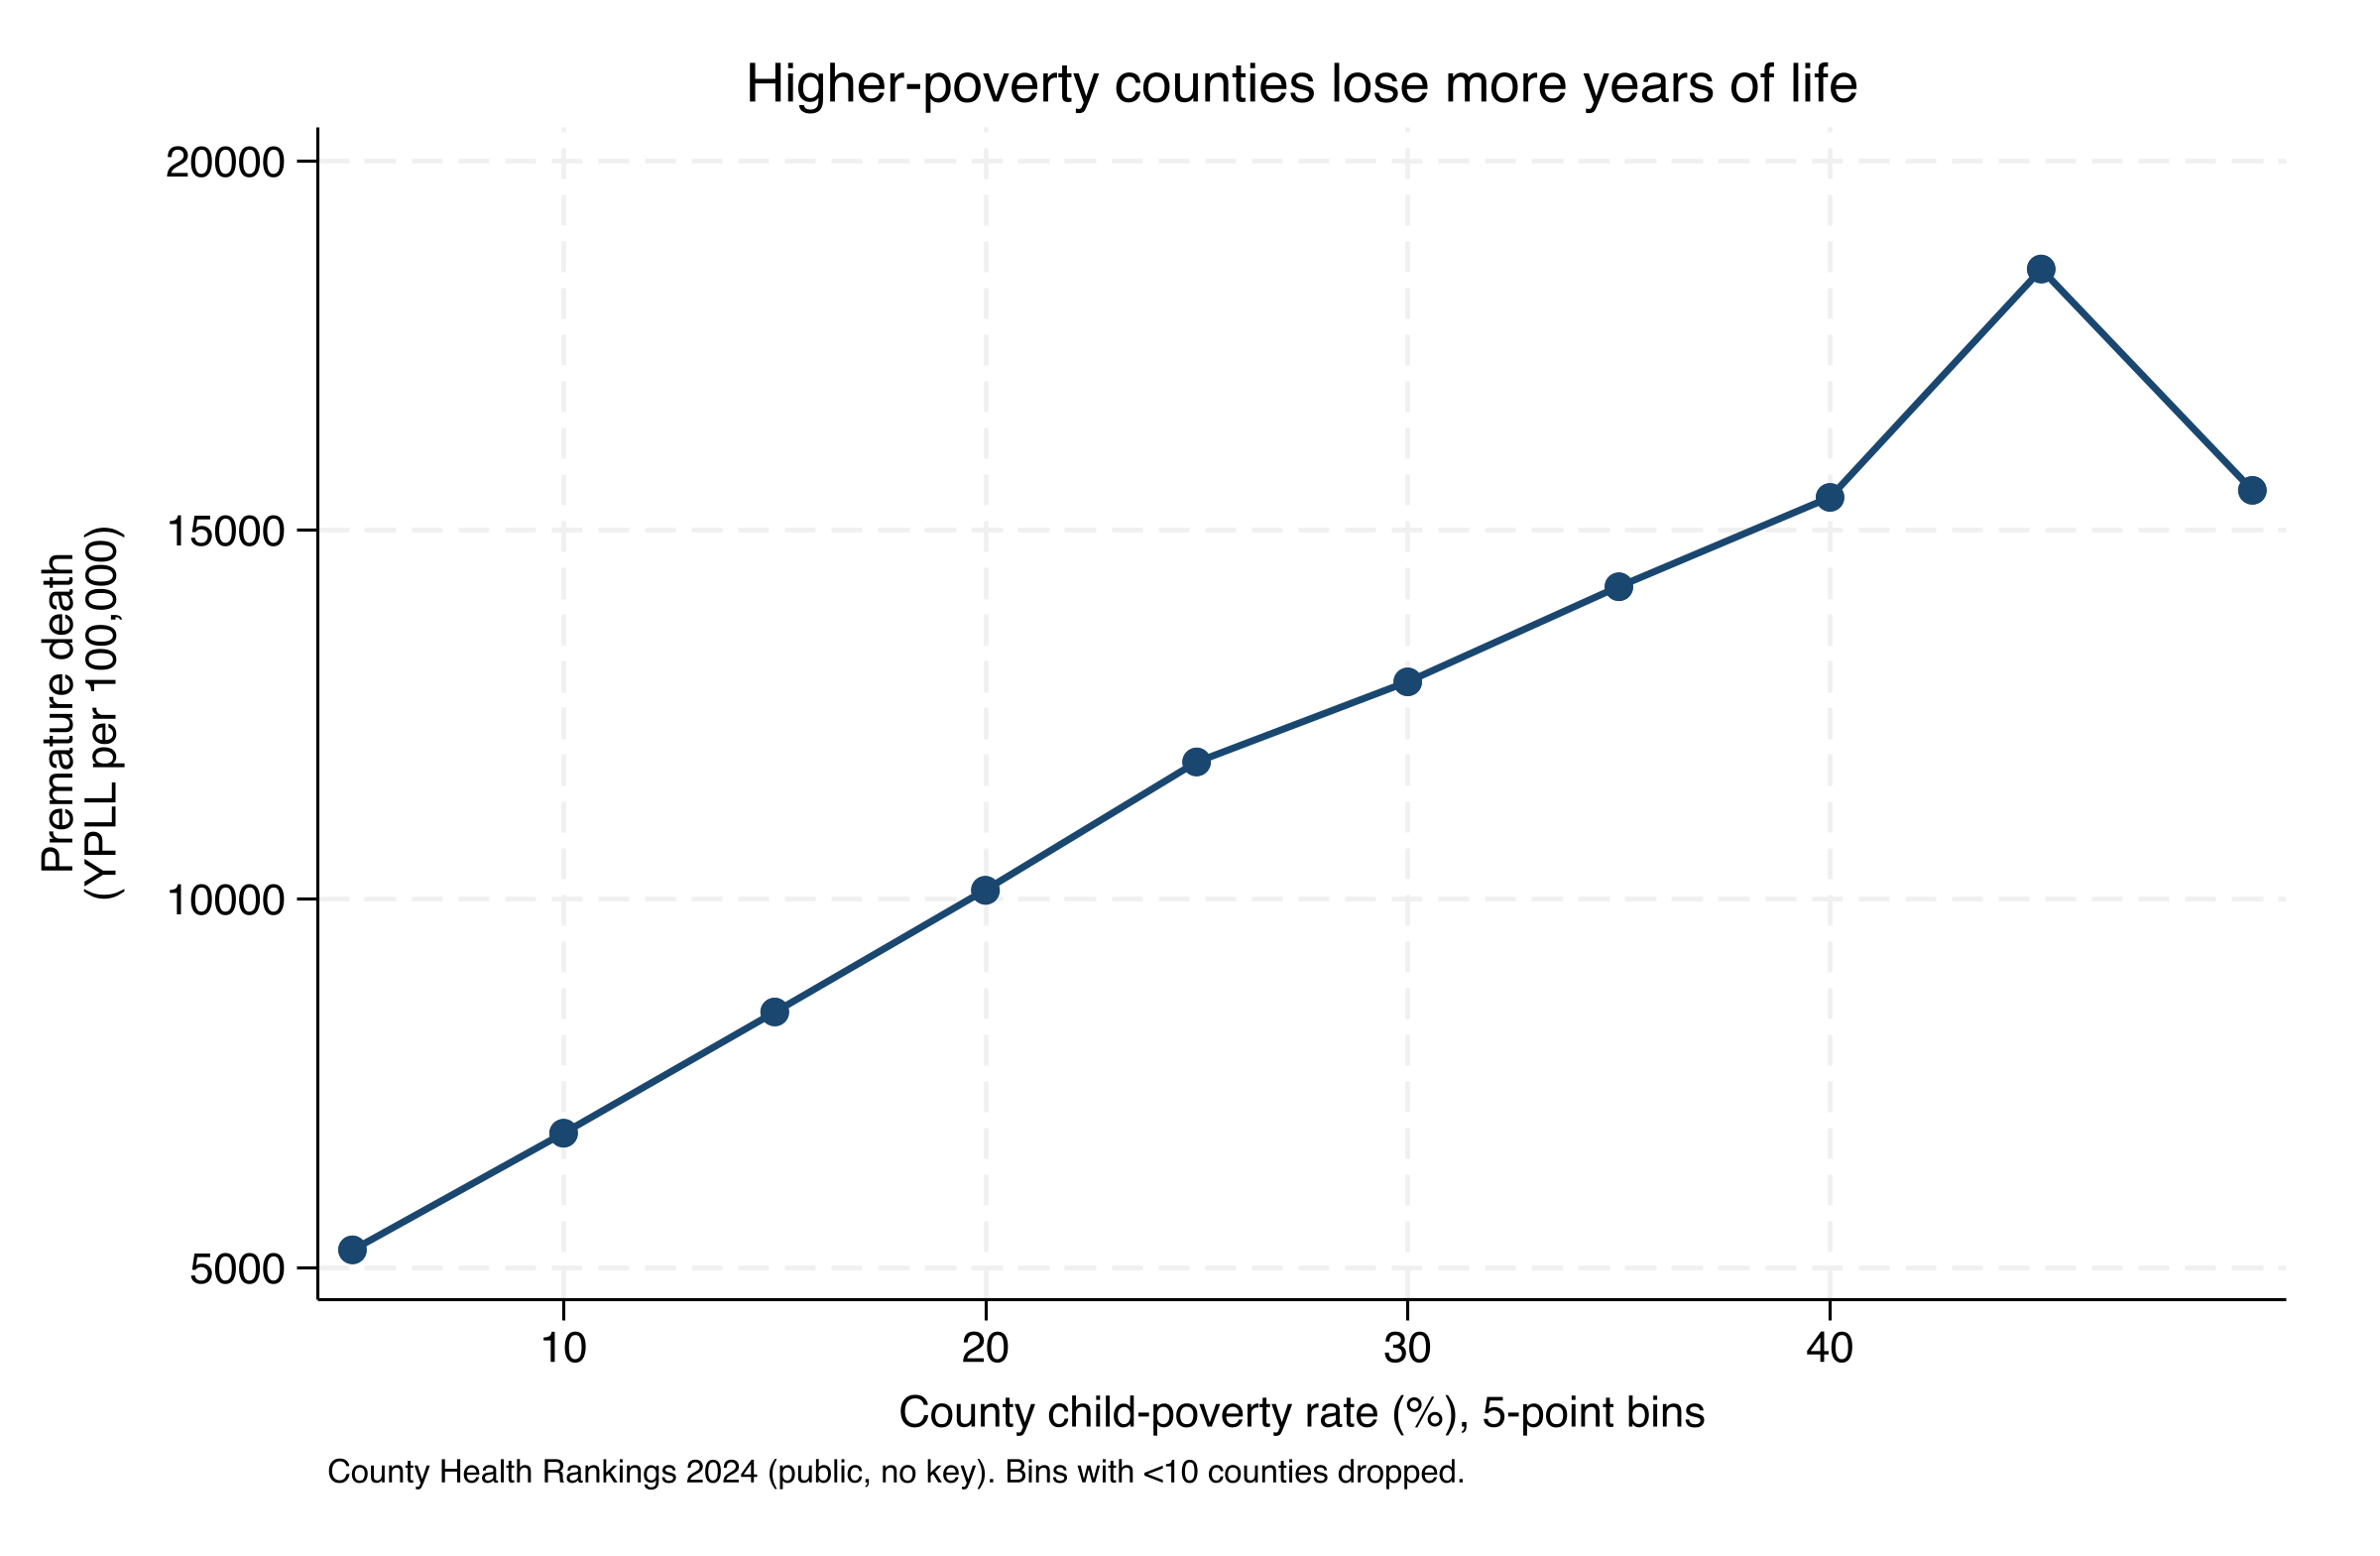
\includegraphics[width=\linewidth]{images/cap_ypll_poverty.png}
\caption{Premature death rises steadily with county child poverty. Each point is the mean YPLL per 100,000 for counties in a five-point poverty bin; we drop bins with fewer than ten counties. A county at 30 percent child poverty averages about 12,900 YPLL, roughly double the 6,800 at 10 percent. County Health Rankings 2024, produced by \texttt{capstone\_chr.do}.}
\label{fig:capstone}
\end{figure*}

\paragraph{Stage 5, visualize (Chapter~\ref{ch:graphs}).} The regression gives one slope; you see the shape behind it more clearly in a picture. The do-file bins counties by poverty rate, averages YPLL within each bin, and plots the means (Figure~\ref{fig:capstone}), and the binned means climb in a near-straight line from the lowest-poverty counties to the highest. Binning is an honest simplification here: it shows the gradient the regression summarizes without asking the reader to trust a single slope, and dropping the thin top bins keeps a handful of tiny counties from reading as a trend.

\paragraph{Stage 6, deliver (Chapters~\ref{ch:sheets}--\ref{ch:portals}).} The do-file ends by shipping the small cleaned extract, not the raw file: it labels the data with the do-file that made it, \texttt{compress}es, and saves \texttt{chr\_2024\_clean.dta}. A collaborator who opens that file can see where it came from and rerun the do-file to remake the figure. That is the replicable principle from Chapter~\ref{ch:embedded} closed in one line.

\paragraph{The honest caveat.} This is a correlation across counties, not a causal claim about people, and not a claim about any one resident. Beware the ecological fallacy: a pattern across counties need not hold across individuals, the same warning attached to Example D.1. What the capstone establishes is narrower and still useful, a defensible, reproducible description of how premature death tracks child poverty across US counties, built the way this book builds everything: guarded, traced to its source, and handed off in a form someone else can run.

\paragraph{Make it yours.} Swap the outcome for a different CHR measure (say, the uninsured-adults rate), or add a third predictor, and rerun. If the county count changes, the \texttt{assert} in Stage~3 will tell you before the regression does. That edit-and-rerun loop, on data you chose, is what keeps the workflow extensible: the structure survives a new outcome or predictor without a rewrite.

\backmatter
\pagelayout{margin}
\chapter{Data Used in This Book}\label{app:data}
Every worked example in this book runs on data you can put your hands on, and this registry is the one place they are all named. The two shipped datasets load with a single command and no download; each public file's entry names its source, so a fresh copy is one URL away; and every simulated dataset states its seed in the do-file that builds it, so the exact numbers in the text rebuild on your machine.

\begin{table*}[htbp]
\centering
\footnotesize
\caption[Datasets used in this book]{Every dataset the book's examples use, where it comes from, and the chapters that use it.}
\label{tab:app-data}
\begin{tabular}{p{3.4cm}p{4.6cm}p{2.6cm}p{2.2cm}}
\hline
Data & Where it comes from & One row per & Chapters \\
\hline
\texttt{auto} & Ships with Stata (\texttt{sysuse auto}); 1978 automobile listings & car model & 4, 5, 8, 9, 12 \\
\texttt{nlsw88} & Ships with Stata (\texttt{sysuse nlsw88}); 1988 NLS extract of working women & woman, age 34--46 & 1, 2, 5, 7, 8, 9, 13, 14 \\
\texttt{nlswork} & Stata's website (\texttt{webuse nlswork}); NLS young women panel, 1968--1988 & woman-year & 6 \\
\texttt{nhanes2f} & Stata's website (\texttt{webuse nhanes2f}); NHANES~II with survey design variables & respondent & 7 \\
County Health Rankings & One national analytic CSV per year from \texttt{countyhealthrankings.org} & county, plus state and national summary rows & 1, 3, 4, 10, 11, 12 \\
Texas Academic Performance Reports & Scraped from the state's download form (Chapter~\ref{ch:noapi}) & campus- or district-year & 4 \\
BLS QCEW & Quarterly wage API at \texttt{data.bls.gov/cew} & county-quarter & 1, 3, 10 \\
Census and ACS endpoints & The API patterns of Chapter~\ref{ch:apis} & varies by pull & 3 \\
Simulated data & Built in each chapter's do-file, \texttt{set seed 20260704} & varies by demonstration & 5, 7, 8, 9, 13, 15 \\
\hline
\end{tabular}
\end{table*}

\pagelayout{margin}

\chapter*{Afterword}
\addcontentsline{toc}{chapter}{Afterword}
Return to the Thursday-afternoon email that opened Chapter~\ref{ch:embedded}: are we reaching the rural students we promised? An answer now begins with the agreed definition of rural, counts each enrolled student once, reports missing locations, and compares the resulting share with the program's target. The analyst retains the source files, code, log, and dated exhibit so a colleague can check the number and repeat the analysis. The four principles describe what the program gains from that work: an answer tied to a decision, a structure that can accept the next data delivery, an explanation the intended audience can understand, and a result another analyst can trace.

Throughout the book, you record consequential choices before seeing the result they can change. The scoping note defines the decision and deadline; the extraction contract records the expected response from a data source; the analysis plan names the comparison; the deliverable specification identifies what the audience will receive; and the disclosure record explains what left the protected environment. In Chapter~\ref{ch:tools}, the syntax statement defines how another researcher will use a command. These records let you explain which choices preceded the analysis and which changed in response to new evidence.

The principles also support one another. A repeatable pipeline reduces the effort needed to add a year or site. A stable structure leaves more time to improve labels, explanations, and the form in which readers receive the result. Readers can then use the work while analysts retain a record of how it was produced. Under a short deadline, begin with the source files, code, and log because later updates and explanations depend on them.

Packages, data endpoints, and hosted LLMs will change after publication. A durable workflow records the software and data version, states the expected result before computing it, and identifies the evidence that would change the conclusion. When an endpoint moves or a definition changes, those records help the next analyst locate the break and decide whether earlier results remain comparable. You can practice that work by rebuilding the capstone with data from your state, checking each assertion, and documenting any changes needed to reproduce the analysis.

The records in an evaluation describe people who answered a survey, enrolled a child, or received a service. Assertions, interpretation caveats, access controls, and disclosure checks protect the quality of the decisions made from their information and reduce the risk that the analysis harms them.

\pagelayout{wide}
\printbibliography[heading=bibintoc, title=Bibliography]

\printindex

\end{document}
